% ****** Start of file apssamp.tex ******
%
%   This file is part of the APS files in the REVTeX 4.1 distribution.
%   Version 4.1r of REVTeX, August 2010
%
%   Copyright (c) 2009, 2010 The American Physical Society.
%
%   See the REVTeX 4 README file for restrictions and more information.
%
% TeX'ing this file requires that you have AMS-LaTeX 2.0 installed
% as well as the rest of the prerequisites for REVTeX 4.1
%
% See the REVTeX 4 README file
% It also requires running BibTeX. The commands are as follows:
%
%  1)  latex apssamp.tex
%  2)  bibtex apssamp
%  3)  latex apssamp.tex
%  4)  latex apssamp.tex
%
\documentclass[%
 reprint,
%superscriptaddress,
%groupedaddress,
%unsortedaddress,
%runinaddress,
%frontmatterverbose,
%preprint,
%showpacs,preprintnumbers,
 nofootinbib,
%nobibnotes,
%bibnotes,
 amsmath,amssymb,
 aps,
%pra,
%prb,
%rmp,
%prstab,
%prstper,
%floatfix,
]{revtex4-1}

\usepackage[caption=false]{subfig}
\usepackage[pass,letterpaper]{geometry}
\usepackage{multirow}
\usepackage{graphicx}% Include figure files
\usepackage{dcolumn}% Align table columns on decimal point
\usepackage{bm}% bold math
\usepackage{longtable}
\usepackage{afterpage}
\usepackage{tabularx}
\usepackage{upquote}
\usepackage{listings}
\usepackage[version=3]{mhchem}
\usepackage[]{SIunits}
\usepackage{multirow}

\lstset{
basicstyle=\small\ttfamily,
columns=flexible,
breaklines=true
breakindent=0pt
}
% Support for subfigure w/ reference


%\usepackage{hyperref}% add hypertext capabilities
%\usepackage[mathlines]{lineno}% Enable numbering of text and display math
%\linenumbers\relax % Commence numbering lines

%\usepackage{showframe}%Uncomment any one of the following lines to test
%%scale=0.7, marginratio={1:1, 2:3}, ignoreall,% default settings
%%text={7in,10in},centering,
%%margin=1.5in,
%%total={6.5in,8.75in}, top=1.2in, left=0.9in, includefoot,
%%height=10in,a5paper,hmargin={3cm,0.8in},
%]{geometry}

\begin{document}

\preprint{APS/123-QED}

\title{
  Monovacancy Properties From Atomistic Simulations Based on OpenKIM
}% Force line breaks with \\
%\thanks{A footnote to the article title}%

\author{Junhao Li}
  \email{jl2922@cornell.edu}
\author{Matt Bierbaum}
\affiliation{
  Department of Physics and Laboratory of Atomic and Solid State Physics\\
  Cornell University, Ithaca, NY 14853, USA
}
\author{Noam Bernstein}
\affiliation{
  Center for Computational Materials Science\\
  Naval Research Laboratory, Washington, DC 20375, USA
}
\author{Ryan Elliott}
\author{Ellad Tadmor}
\affiliation{
  Department of Aerospace Engineering and Mechanics\\
  University of Minnesota, Minneapolis, MN 55455, USA
}
\author{James P. Sethna}
  \email{sethna@lassp.cornell.edu}
\affiliation{
  Department of Physics and Laboratory of Atomic and Solid State Physics\\
  Cornell University, Ithaca, NY 14853, USA
}
%\author{Ann Author}
% \altaffiliation[Also at ]{Physics Department, XYZ University.}%Lines break automatically or can be forced with \\
%\author{Second Author}%
% \email{Second.Author@institution.edu}
%\affiliation{%
% Authors' institution and/or address\\
% This line break forced with \textbackslash\textbackslash
%}%
%
%\collaboration{MUSO Collaboration}%\noaffiliation
%
%\author{Charlie Author}
% \homepage{http://www.Second.institution.edu/~Charlie.Author}
%\affiliation{
% Second institution and/or address\\
% This line break forced% with \\
%}%
%\affiliation{
% Third institution, the second for Charlie Author
%}%
%\author{Delta Author}
%\affiliation{%
% Authors' institution and/or address\\
% This line break forced with \textbackslash\textbackslash
%}%
%
%\collaboration{CLEO Collaboration}%\noaffiliation

\date{\today}% It is always \today, today,
             %  but any date may be explicitly specified

\begin{abstract}
In this paper, we describe how we obtain the monovacancy properties for all the elements and all the simple crystal structures predicted by the hundreds of interatomic potential models on OpenKIM, the knowledgebase of interatomic models.
The properties we calculated include the vacancy formation energy, migration energy, relaxation volume, elastic dipole tensor, defect strain tensor, and saddle point elastic dipole and defect strain tensors.
The structures we calculate include sc, fcc, bcc, diamond, and hcp.
These results can provide use information for selecting interatomic models.
We also examine how these properties depend on each other and other elemental properties.

%An article usually includes an abstract, a concise summary of the work
%covered at length in the main body of the article.
%\begin{description}
%\item[Usage]
%Secondary publications and information retrieval purposes.
%\item[PACS numbers]
%May be entered using the \verb+\pacs{#1}+ command.
%\item[Structure]
%You may use the \texttt{description} environment to structure your abstract;
%use the optional argument of the \verb+\item+ command to give the category of each item.
%\end{description}
\end{abstract}

%\pacs{Valid PACS appear here}% PACS, the Physics and Astronomy
                             % Classification Scheme.
%\keywords{Suggested keywords}%Use showkeys class option if keyword
                              %display desired
\maketitle

%\tableofcontents

\section{\label{sec:intro}Introduction}

A longtime goal of scientists' is to be able to calculate the properties of materials from their structures accurately and efficiently.
There are several approaches to this problem, including the density functional theory (DFT) and the atomistic simulation.
DFT has developed rapidly in the recent few decades and achieved decent accuracy for many small-scale systems.
However, in many cases, the size, the complexity, or the timescale we want to simulate, demands a much more efficient method.
And atomistic simulation with good interatomic potentials is one of the methods that can fulfill this demand.

Several different types of interatomic models have been developed over the past few decades, from pairwise models like Lennard-Jones, to those based on cluster functionals such as the embedded-atom method (EAM) \cite{daw1993embedded, daw1984embedded}.
One problem that has hindered the development of atomistic simulation is that the models developed by various researchers are usually presented in different formats, making them difficult to reuse.
The OpenKIM project \cite{bierbaum2014openkim, openkim2016} solves this problem by providing a unified framework for model developers to submit, and for model users to perform atomistic simulations \cite{tadmor2011potential}.
It also hosts a repository of reference data from other sources, such as DFT and experiments, for assessing the quality of these models.
% sample elements from the whole periodic table and various structures and find out or discover suitable materials and structures in an automated way, which in the past could only be done with DFT \cite{ceder2010opportunities, zhou2010iron,norskov2009towards} and thus was only applicable for small structures.

In this study, we focus on vacancies, the simplest and the most common point defects.
Finding interatomic models that can accurately describe vacancy effects is extremely beneficial for furthering our understanding and application of materials.
Vacancies mediate dislocation climb and creep \cite{weertman1955theory} and the diffusion of substitutional defects \cite{fahey1989point}.
They are also the dominant flow mechanism under external fields, such as gravity \cite{sethna2014flow}.
And in metrology, some scientists propose to use \ce{^{28}Si} for a new definition of kilogram, and obtaining the equilibrium vacancy concentration is a crucial part of this work \cite{andreas2011counting}.
% As mentioned in their report, they have achieved an accuracy below $5~\mu\gram$ in the $1~\kilogram$ mass determination, and the point defect correction is as large as $24.3(3.3)~\mu\gram$ \cite{andreas2011counting}.

% FROM JIM EMAIL

Defects in crystals not only have a free energy, describing the cost of formation, but they also have an environmental impact through the generation of long-range fields.
Cracks have mode~I, mode~II, and mode~III stress and strain fields; dislocations have strain fields determined by their orientation and Burger's vector, and so on.
The long-range electrical impact of a point defect is described at lowest order by its charge, and to higher order by by a charge multipole series;
the long-range magnetic impact is partly the direct dipolar interaction between local moments and mostly the RKKY-type interactions mediated by conduction electrons.
Neither of these are part of the current KIM potentials, although there are plans to incorporate charge states of atomic species in the next release.
The long-range elastic environmental impact of our vacancies will thus be described at lowest order by the {\em elastic dipole} field -- a strain field induced by the vacancy that dies $1/R^3$ like the electrical dipole field.%
\footnote{
There is a nomenclature problem in the field.
The anisotropic part of the $1/R^3$ elastic field around a defect in an isotropic medium has the $L=2$ symmetry of an electrical quadrupole, and is often described as the elastic quadrupole field.
But calling the isotropic part a monopole field would be strange since it also decays as $1/R^3$.
We believe neither choice is very satisfactory, but the alternative of naming it after Eshelby seems strange as well.
}
We thus calculate these elastic dipole fields, as well as the vacancy creation energy.

Each defect will have an environmental dependence as well.
Vacancies in electric fields have a direct Coulomb force in insulators, and an important electromigration forces from the `electron wind' in metals (which may be in the opposite direction from the electrical current); neither is accessible in the current KIM potentials.
The pressure dependence of the vacancy creation energy, and the energy change due to external stresses, will be given by its elastic dipole field (discussed above).
Our vacancy will diffuse due to pressure gradients and concentration gradients, with a rate given by the free energy barrier to motion (which we also calculate).
In turn, the pressure or stress dependence of the free energy will be determined by the difference between the vacancy's elastic dipole in the ground state and at the saddlepoint for the motion, which we also calculate.
The entropic effects of vibrations at the ground state and saddlepoint, needed for the complete transition-state estimate for the prefactor of the diffusion constant~\cite{burada2009diffusion}, will in general depend upon whether the system described is a classical simulation or a quantum solid, and goes beyond the purview of our work here.

% END FROM JIM


In order to assess how each interatomic potential model performs in vacancy-related simulations, we calculate the most important monovacancy properties for all the elements and all the simple crystal structures predicted by the interatomic potential models available on OpenKIM at this time.
The properties we calculate include the vacancy formation energy (VFE), the vacancy migration energy (VME), the vacancy relaxation volume (VRV), the elastic dipole tensor (EDT), the defect strain tensor (DST), and the saddle point elastic dipole tensor (SPEDT) and defect strain tensor (SPDST).
VFE and VME give us the local energy change.
VRV and the four tensors describe the long-range environmental impact.
The OpenKIM website properties page\footnote{OpenKIM website properties page url: \url{https://openkim.org/properties}} provides a brief description to these quantities.
Sec.~\ref{sec:method} describes the method we used to obtain these quantities.
The structures we calculate include sc, fcc, bcc, diamond, and hcp.
The results can be compared with data from other sources, such as the density function theory (DFT), the quantum Monte Carlo (QMC), and the experiments, and provide use information when selecting interatomic models for vacancy-related simulations.
They can also be used with continuum models to obtain an initial guess for further atomistic simulations \cite{bozhevolnyi2001multiple}.
In this paper, we compare our VFE and VME results for fcc and hcp structures to DFT calculations and experiments \cite{angsten2014elemental}.
% We found that EAM potentials, in general, provide results closer to these reference data then other models at this time.

In addition, we explored how these properties relate to each other, and to other elemental properties, such as the cohesive energy and the bulk modulus.
Both the vacancy formation energy and the vacancy migration energy show linear correlation with the cohesive energy, with slopes of $0.32\pm0.04$ and $0.14\pm0.04$ respectively.
The migration energy and the relaxation volume are correlated with the bulk modulus, the first with a positive slope of $(0.57\pm0.03)\angstrom^3$, and the second with a negative slope of $(-4.2\pm0.7)\angstrom^6\per\electronvolt$.
All of these results are consistent with physics intuition and previous literature \cite{angsten2014elemental}.
These relationships can provide additional information in selecting models and screening structures.

The paper is organized as follows.
In Sec.~\ref{sec:method} we describe the method we use for calculating the monovacancy properties.
In Sec.~\ref{sec:results} we show the plots of our results, compare them with the reference data, and explore how they relate to each other and to other elemental properties.
And Sec.~\ref{sec:conclusion} concludes this paper.

\section{\label{sec:method}Methodology}

In this section, we explain how we calculate the monovacancy properties, including the vacancy formation energy (VFE), the vacancy migration energy (VME), the vacancy relaxation volume (VRV), the elastic dipole tensor (EDT), the defect strain tensor (DST), and the saddle point elastic dipole tensor (SPEDT) and defect strain tensor (SPDST).
For a brief description of these quantities, you can check the OpenKIM website properties page.

The calculation is based on OpenKIM \cite{openkim2016} and the Atomic Simulation Environment (ASE) \cite{bahn2002object}.
The code can be found in the OpenKIM repository with ID \lstinline{TD_000000000000} (TODO).
Here, we discuss the method we used for obtaining each of these quantities.

The free energy per unit volume of a crystal can be described by the following equation \cite{freedman2009elastic}
\begin{equation}\label{eq:f}
f = f_0 + n_dE_d + \frac{1}{2}n_d^2E_{dd} + \frac{1}{2}C_{ijkl}\epsilon_{ij}\epsilon_{kl} - n_d\epsilon_{ij}G_{ij}
\end{equation}
where $n_d$ is the defect concentration, $\epsilon_{ij}$ is the bulk strain, $E_d$ is the vacancy formation energy, $E_{dd}$ describes the energy from defect interaction, $C_{ijkl}$ is the elastic stiffness tensor, and $G_{ij}$ is the elastic dipole tensor.
$f_0$ is the chemical potential. If $n$ is the number of atoms per unit volume and $E_0$ is the cohesive energy per atom corresponding to a perfect crystal (what we defined as the reservoir), then $f_0 = (n - n_d) E_{0}$.

It is worthwhile to examine the physical meaning behind each term.
We assume the vacancies only interact with each other through the strain field and that the nonlinear behavior of the elasticity is negligible.
Then for a unit volume, the total cohesive energy can be described by
\begin{equation}
\label{eq:f_explain}
f =  \int_V E_{\mathrm{chemical}} + \frac{1}{2}C_{ijkl}\widetilde{\epsilon}_{ij}\widetilde{\epsilon}_{kl} dV
\end{equation}
Here $\widetilde{\epsilon}$ is the strain corresponds to each $dV$, which consists of the bulk strain $\epsilon$, the strain caused by the nearest vacancy $\widetilde{\epsilon}_V$ and other vacancies $\widetilde{\epsilon}_I$.
\begin{equation}
  \widetilde{\epsilon}_{ij} = \epsilon_{ij} + \widetilde{\epsilon}_{V,ij} + \widetilde{\epsilon}_{I,ij}
\end{equation}
Thus
\begin{align}
  \widetilde{\epsilon}_{ij}\widetilde{\epsilon}_{kl}
  = & \epsilon_{ij}\epsilon_{kl} + \widetilde{\epsilon}_{V,ij}\widetilde{\epsilon}_{V,kl}
  + 2\epsilon_{ij}\widetilde{\epsilon}_{V,kl}
  + I(\epsilon, \widetilde{\epsilon}_{V}, \widetilde{\epsilon}_{I})
\end{align}
The first term is the energy due to the bulk strain.
The second term together with the change in $E_\mathrm{chemical}$ give $E_d$.
Since both of them peak at the vacant sites and drop rapidly when moving away, $\partial f /\partial E_d \propto n_d$.
The third term gives how the formation energy change with respect to the bulk strain, and thus represents $G$.
For the similar reason as mentioned above, $\partial f/\partial G \propto n_d$.
And the last term, which includes all the remaining terms in the expansion, represents the interaction $E_{dd}$.
To see how the total interaction energy changes, we first notice the strength of $\widetilde{\epsilon}_I$ is proportional $n_d$ because of the strain obeys the superposition principle in linear elasticity.
In addition, note that if the vacant sites form a Bravais lattice, which is the configuration we are using in our calculation, the peak of these $\widetilde{\epsilon}_I$ will also occur on these lattice points.
Therefore the number of peaks is proportional to $n_d$ as well.
So the overall interaction energy, to the lowest order approximation, is related to $f$ by $\partial f/\partial E_{dd} \propto n_d^2$.

From Eq.~(\ref{eq:f}), the negative derivative of $f$ with respect to $n_d$ under zero strain gives the vacancy formation energy
\begin{equation}
  \label{eq:VFE0}
  \mathit{VFE} = E_d = \left.\frac{\partial f}{\partial n_d}\right|_{\epsilon = 0} + E_{0} - n_d E_{dd}
\end{equation}
Numerically, we use the supercell approach.
For a supercell of volume $V_0$ with a monovacancy, $n_d=1/V_0$, Eq.~(\ref{eq:VFE0}) is equivalent to
\begin{equation}
  (E_{V_0, d} - E_{V_0}) + E_{0} = \mathit{VFE} + \frac{E_{dd}}{V_0} \stackrel{\mathrm{def}}{=} \mathit{g}(V_0)
\end{equation}
Here $E_{V_0, d}$ and $E_{V_0}$ are the free energy of the supercell with and without the defect respectively.
And we define the expression in the middle as $g(V_0)$, thus $\mathit{VFE} = g(\infty)$.
We obtain this $g(\infty)$ through extrapolation.
The uncertainty of this value is the root sum square of the uncertainty from the extrapolation and the uncertainty from the atomistic relaxation.


The negative derivative of $f$ with respect to strain gives the stress
\begin{equation}
  \label{eq:stress}
  \sigma_{ij} = -\frac{\partial f}{\partial \epsilon_{ij}}
  = -C_{ijkl}\epsilon_{kl} + n_dG_{ij} - \frac{1}{2}n_d^2\frac{\partial E_{dd}}{\partial \epsilon_{ij}}
\end{equation}
And the derivative of $\sigma_{ij}$ with respect to $n_d$ with fixed strain $\epsilon_0$ gives the elastic dipole tensor
\begin{equation}
  \label{eq:EDT}
  G_{ij} = \left.\frac{\partial \sigma_{ij}}{\partial n_d}\right|_{\epsilon = \epsilon_0}
  + n_d \left.\frac{\partial E_{dd}}{\partial \epsilon_{ij}}\right|_{\epsilon = \epsilon_0}
\end{equation}
Similarly, we obtain the value and the uncertainty of EDT through extrapolation.

The defect strain tensor $\Lambda_{ij}$ is obtained by
\begin{equation}
  \label{eq:DST}
  \Lambda_{ij} = S_{ijkl} G_{kl}
\end{equation}
where $S_{ijkl}$ is the elastic compliance tensor, which is the inverse of the elastic stiffness tensor $C_{ijkl}$.

The relaxation volume, VRV, is the decrease in the volume of the material due to the monovacancy.
There are two methods for calculating this quantity.
One is through relaxing both the positions of the atoms and the size of the supercell.
And the other is through its relationship with the defect strain tensor.
For an orthorhombic supercell
\begin{equation}
  \label{eq:VRV}
  \mathit{VRV} = V_0\epsilon_{ii} = \Lambda_{ii}
\end{equation}
We verified that these two methods give consistent results.
Since the second method does not involve additional relaxation, we use that one in our calculation.
Note that the supercells used in our calculation for different structures are all orthorhombic cells.
For sc, fcc, bcc, and diamond structures, we use the conventional cubic cell as the basis for constructing supercells, and for hcp structures, we use the one with lattice vectors $(a, \sqrt{3}a, c)$ as the basis.

For vacancy migration, we use the nudged elastic band method to obtain the migration path and cubic spline interpolation to obtain the saddle point energy and configuration.
We use a similar extrapolation method to obtain the vacancy migration energy (VME) and the saddle point elastic dipole and defect strain tensors.
Since the configuration of the saddle point is still a monovacancy, the quantities shall scale in the same way with respect to the number of atoms.

\begin{figure}
\centering
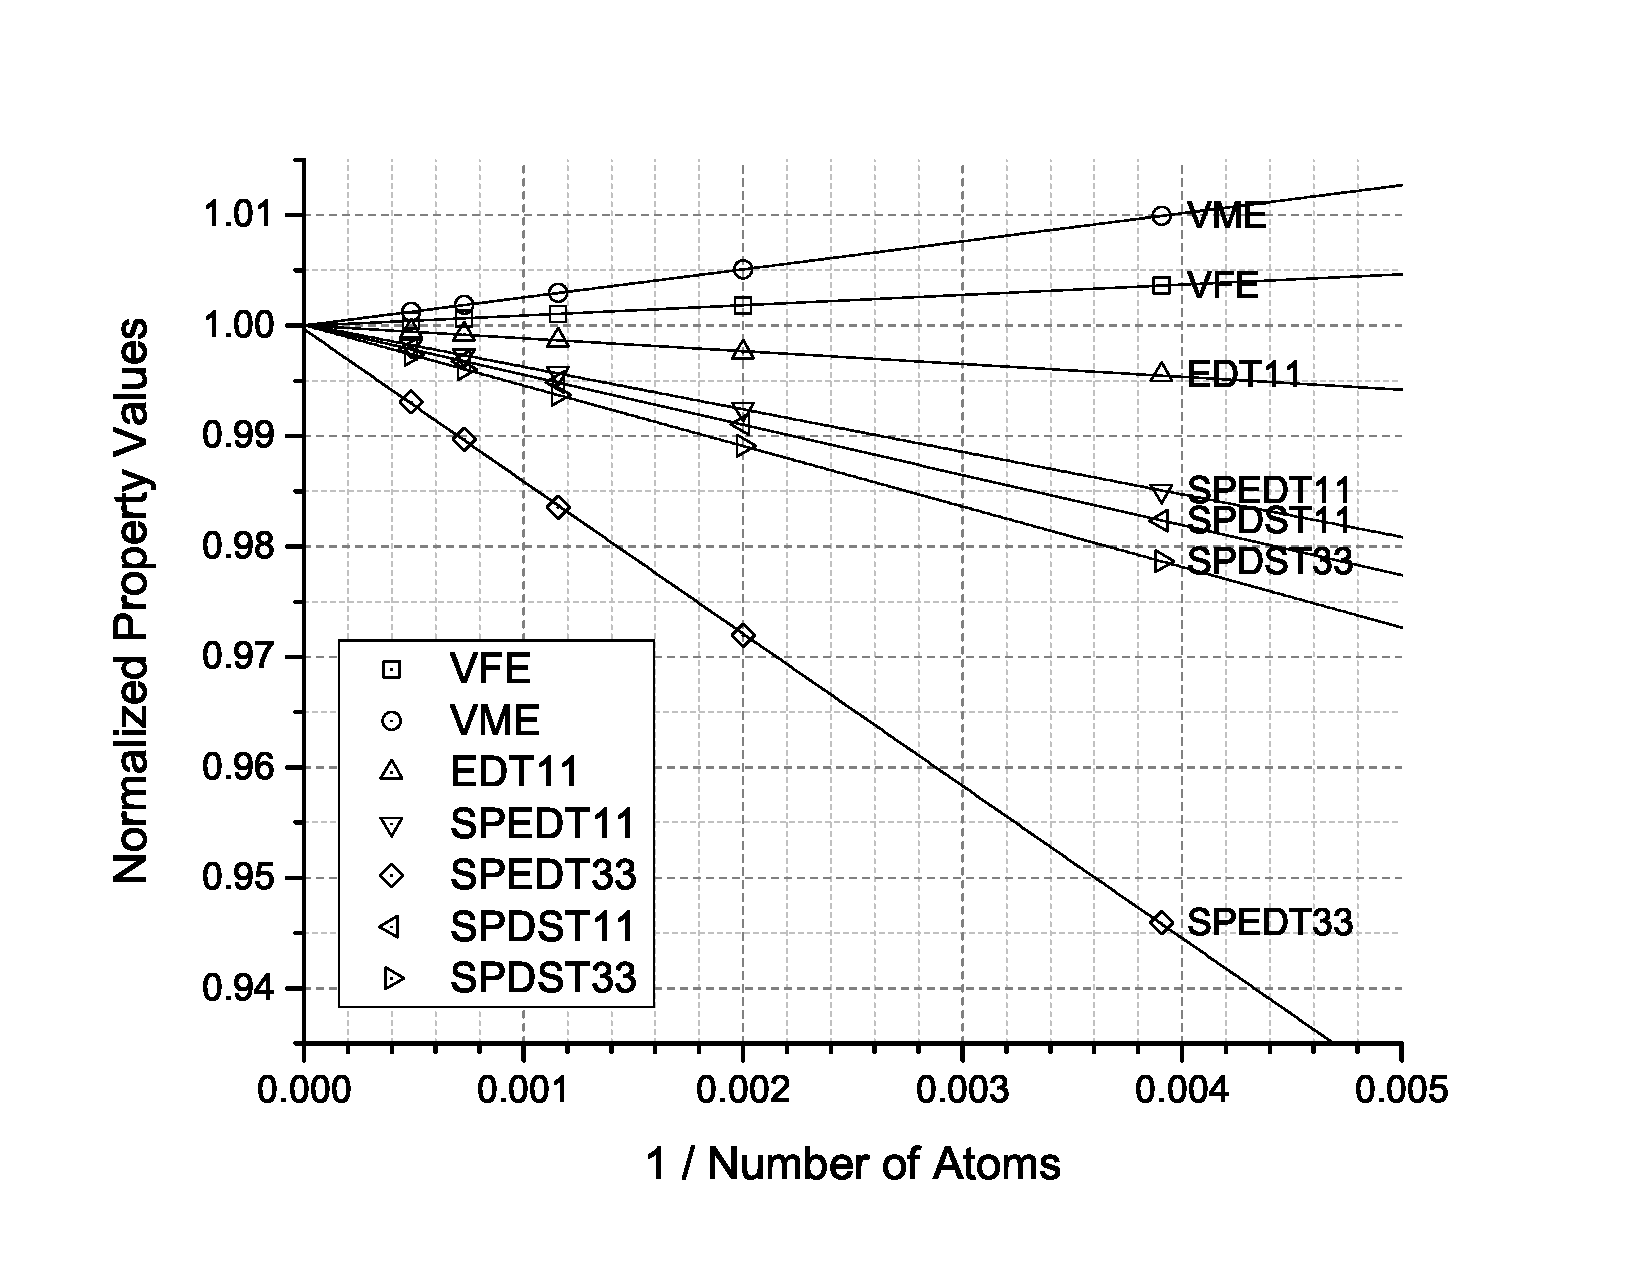
\includegraphics[width=0.5\textwidth, clip, trim = 10mm 10mm 10mm 10mm]{extrapolation2}% Here is how to import EPS art
\caption{\label{fig:extrapolation}
Property values normalized by the extrapolated values versus the inverse of the number of atoms in a supercell.
These values are calculated for fcc aluminum with the embedded atom model (EAM) from Mishin and Farkas \cite{mishin1999interatomic}.
The migration path is from (0.0, 0.0, 0.0) to (0.5, 0.5, 0.0) in a conventional fcc unit cell.
VFE is the vacancy formation energy, VME is the vacancy migration energy, VRV is the vacancy relaxation volume, EDT is the elastic dipole tensor, DST is the defect strain tensor, and SP stands for the saddle point of the migration.
The two numbers following the tensor are the row and column indices.
Since VRV and DST11 are all proportional to EDT11, they will appear as the same curve after normalization, so we show EDT11 here only.
EDT22 and EDT33 are the same as EDT11, and all the off-diagonal terms of EDT are zero.
So are the terms in DST.
The linear relationship shown in this figure validates our extrapolation.
In order to avoid crowding the graph, the error bars are not shown here.
}
\end{figure}

In Fig.~\ref{fig:extrapolation}, we plot the normalized property values for fcc aluminum versus the number of atoms in a supercell, calculated with the embedded atom model (EAM) by Mishin and Farkas \cite{mishin1999interatomic}.
The linear relationship shown in this figure validates our extrapolation.

The calculated results can be found in the OpenKIM repository \cite{openkim2016}.
Appendix~\ref{app:data} provides scripts for retrieving these results.

A key quantity in these results that distinguishes different vacancies and migrations is the position of the vacancy.
In the simplest case where symmetry is preserved, this is unambiguously the position of the center of the symmetry.
However, in complex crystals or vacancies that break symmetries, there is no unique definition for the position of a vacancy.
We propose the following definition, optimized for use in continuum calculations:
The position of the vacancy (or any point defect) is the point, where, if we characterize the effect of the defect as a series of force multipoles at this point, the diagonal terms of the force quadruple are zero in the basis that diagonalizes the force dipole.
Appendix~\ref{app:position} provides a more detailed explanation.
This has been adopted as the KIM property definition for vacancy position.

\section{\label{sec:results}Results and Discussion}

All the results calculated in this work are available in the OpenKIM repository \cite{openkim2016} and can be either viewed directly on the website or downloaded through OpenKIM Query with the scripts provided in Appendix~\ref{app:data}.

In this section, we first compare these results with the reference data to see how these models perform in general.
We then explore how these quantities related to each other and to other elemental properties.

\subsection{\label{sec:calcvsref}Calculated Results Versus Reference Data}

Fig.~\ref{fig:compare} compares our results and with the reference data from DFT calculations and experiments.

\noindent\begin{figure*}
\centering
\noindent\ignorespaces
\subfloat[][]{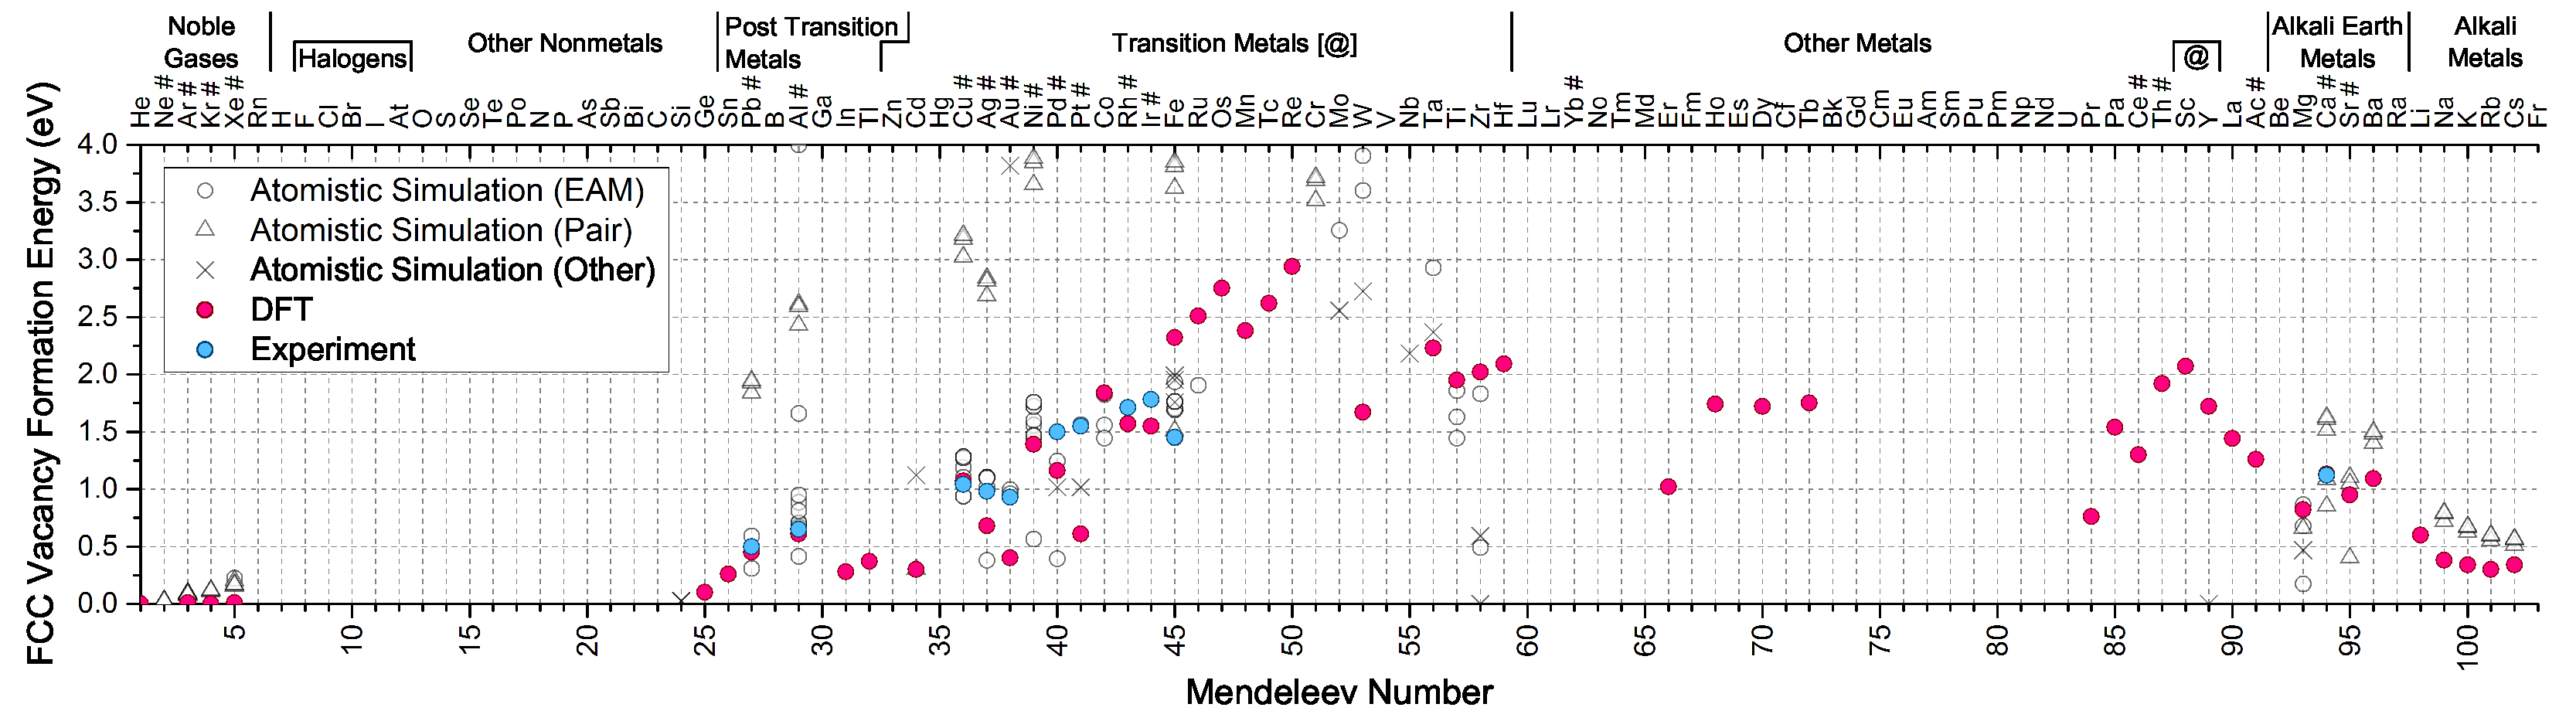
\includegraphics[trim=0 0 0 0,clip,width=1.0\textwidth]{fcc_vfe_new}}
\newline
\subfloat[][]{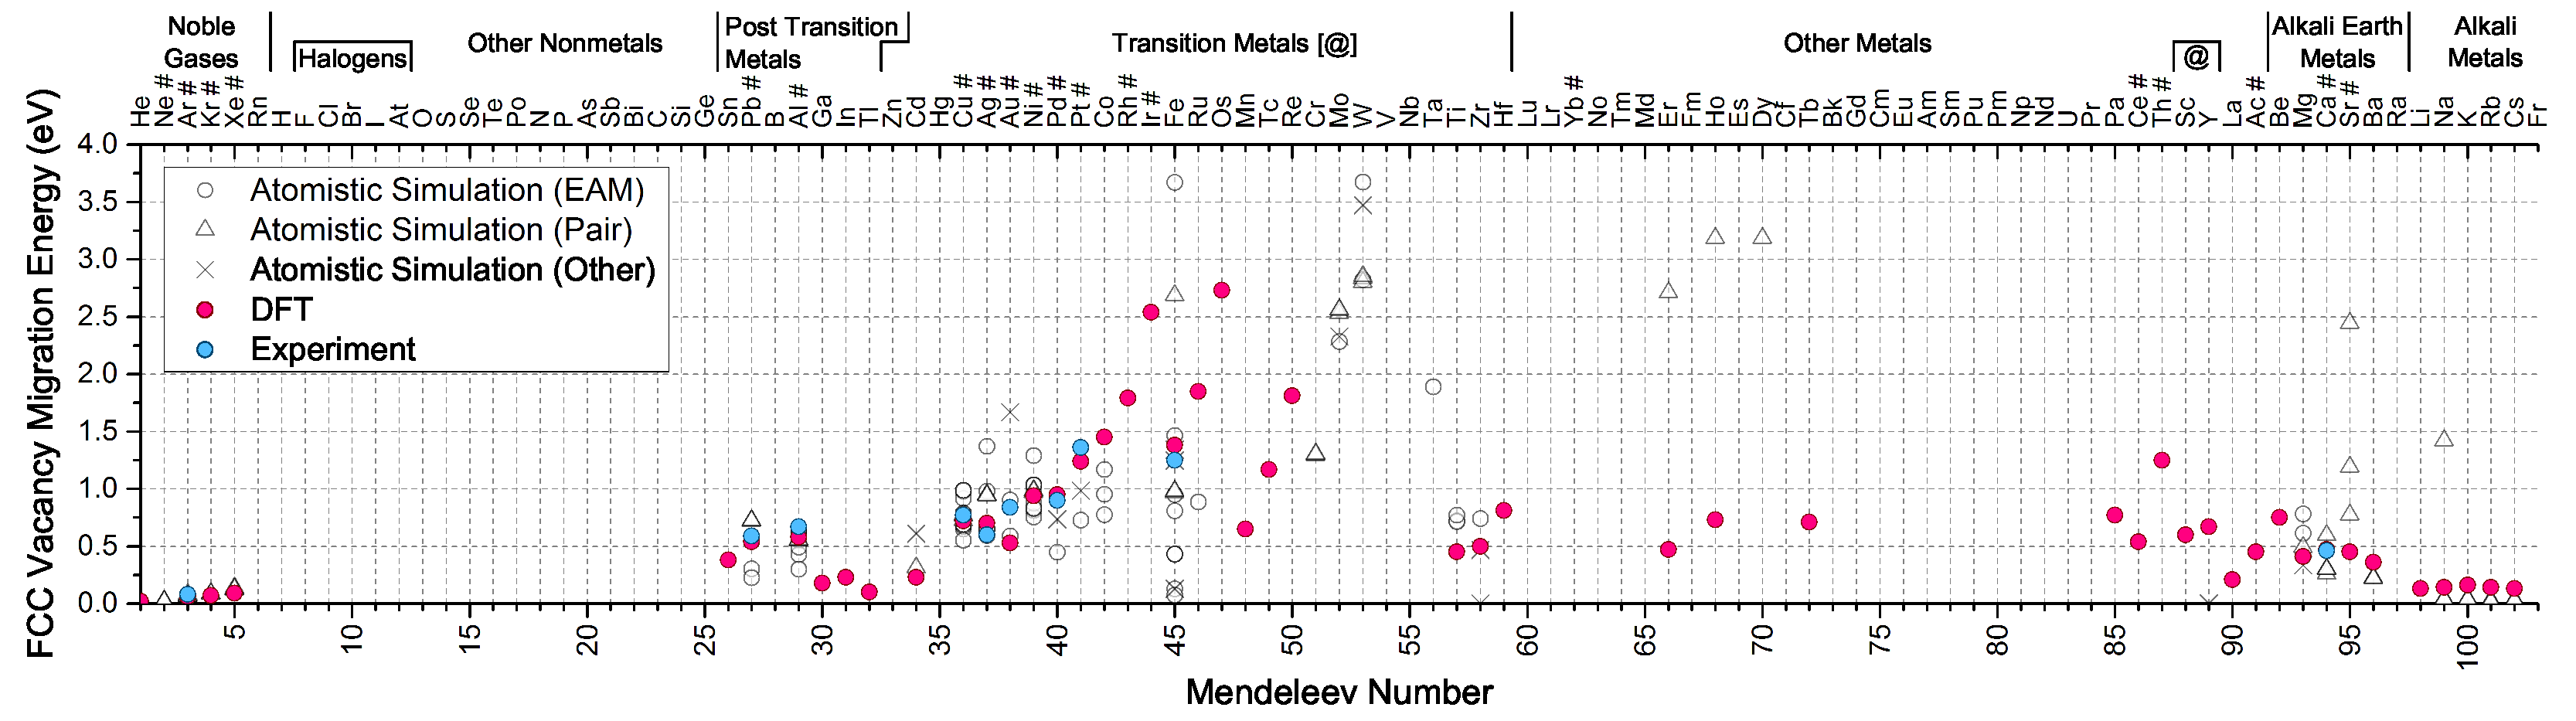
\includegraphics[trim=0 0 0 0,clip,width=1.0\textwidth]{fcc_vme_new}}
\newline
\subfloat[][]{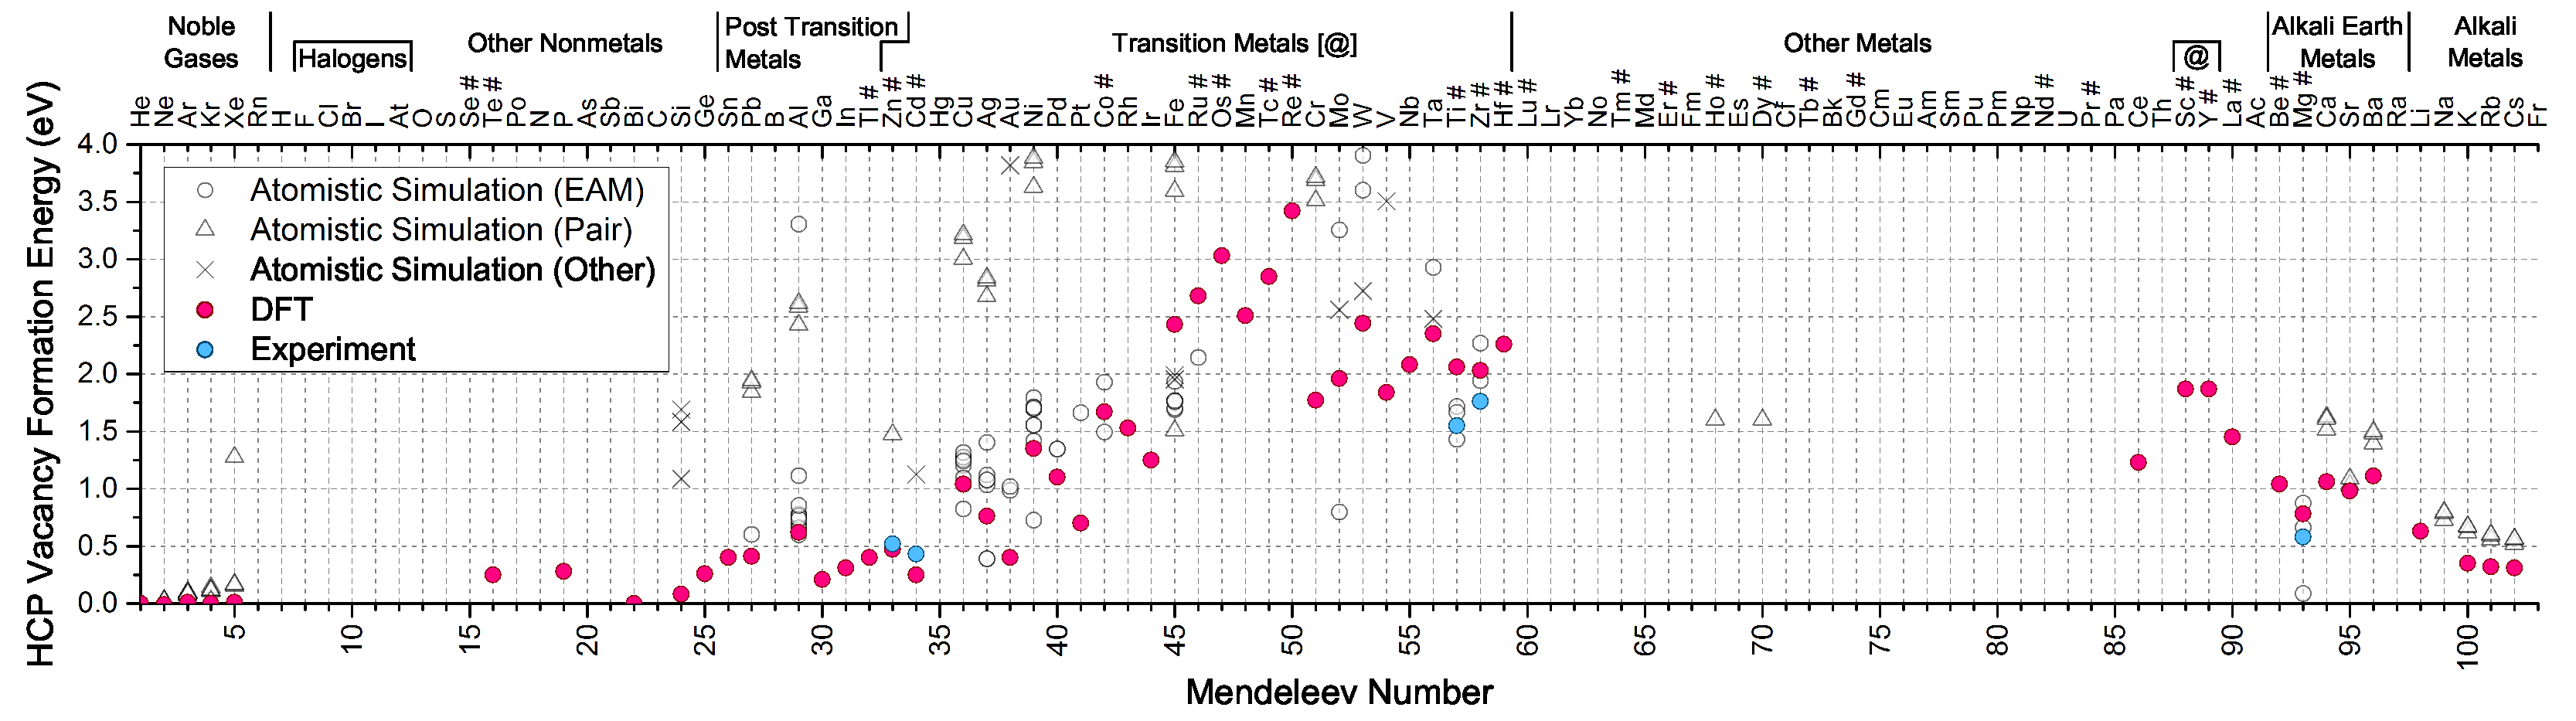
\includegraphics[trim=0 0 0 0,clip,width=1.0\textwidth]{hcp_vfe_new}}
\newline
\subfloat[][]{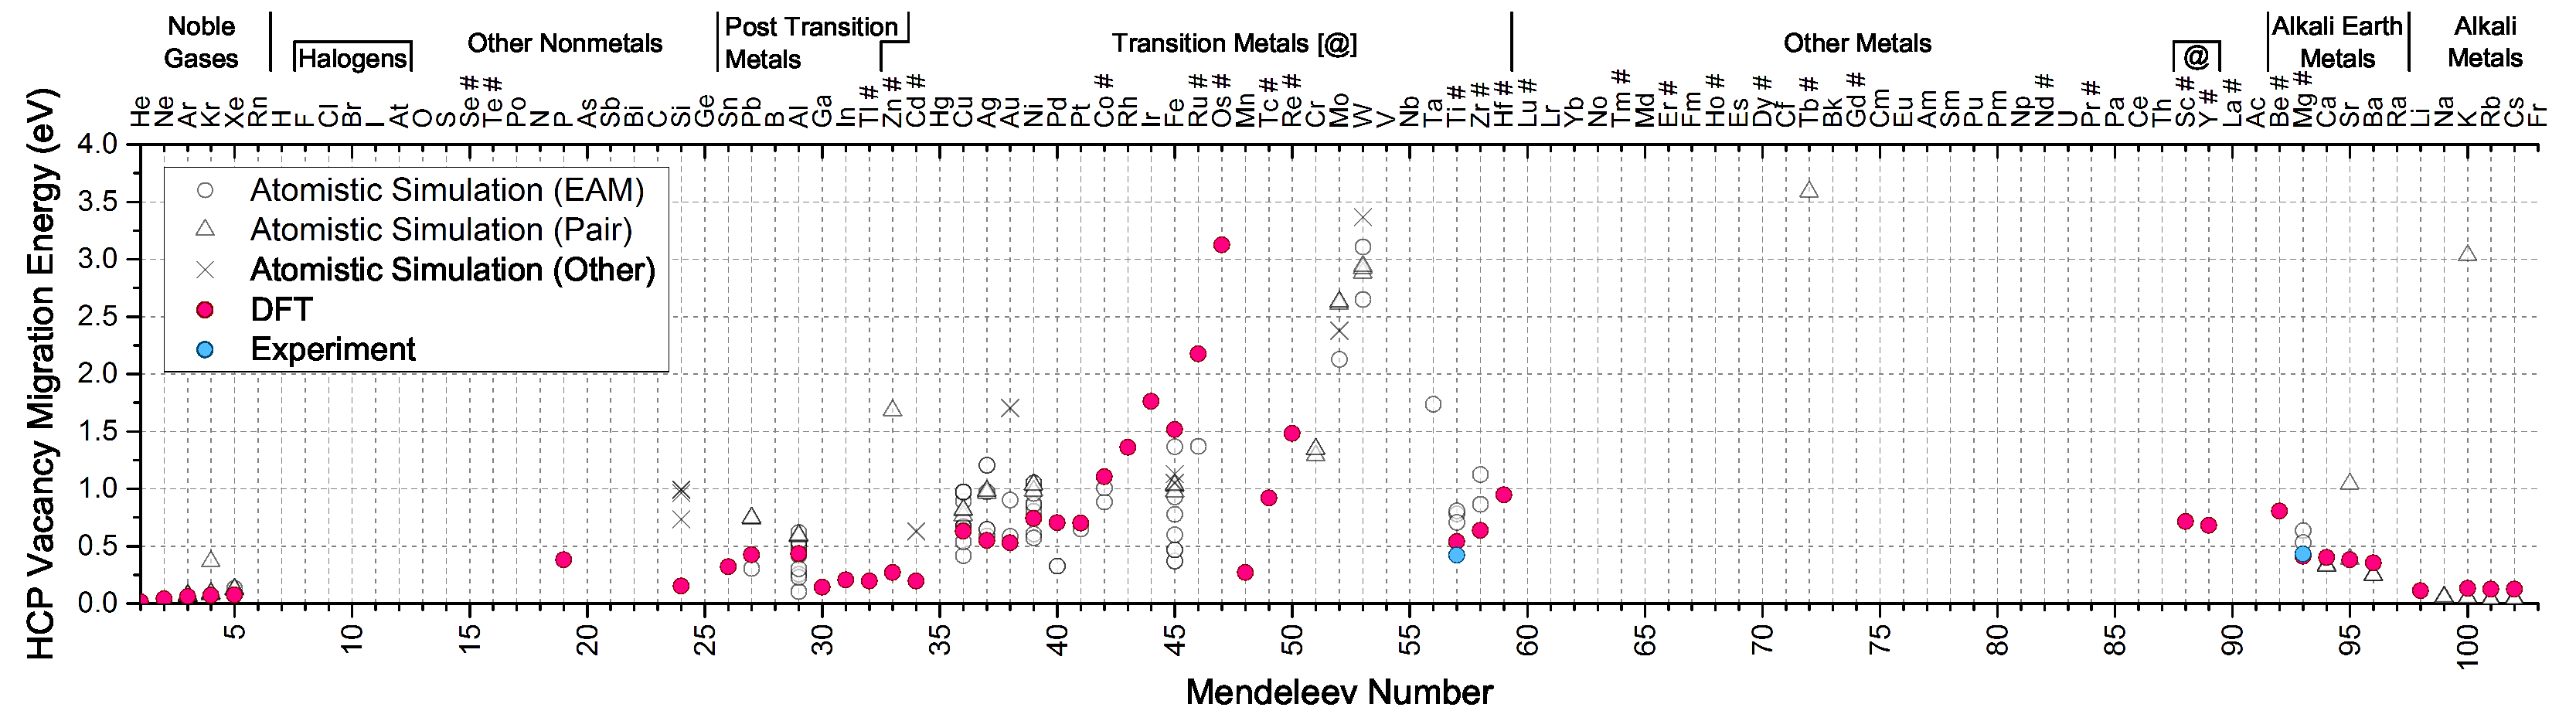
\includegraphics[trim=0 0 0 0,clip,width=1.0\textwidth]{hcp_vme_new}}
\caption{\label{fig:compare}
 Comparison with the reference data.
 % where Fig.~(a) and (b) are the results for fcc structures, and Fig.~(c) and (d) are the results for hcp structures.
 The `\#' sign next to the symbol of each element indicates whether the structure presented in the figure is the element's natural state.
 The error bars are smaller than the size of the symbols.
 See the OpenKIM model page for an interactive interface allowing investigation of the individual potentials for each symbol shown.
}
\end{figure*}

We can see from these figures that the EAM models, in general, produce similar VFE and VME as DFT calculations and experiments.
While most pairwise models tend to produce larger values for VFE, especially for elements with Mendeleev numbers ranging from 25 to 45, which correspond to the transition metals and the post-transition metals.

To further explore how pairwise models come up with larger VFEs, we used fcc aluminum as an example and looked into the relationships between its cohesive energy $E_0$, unrelaxed vacancy formation energy $E_u$, and relaxed vacancy formation energy $E_r$.
We found that, with a pairwise potential (Morse), $E_0 = 2.70\electronvolt \approx E_u$.
While with an EAM potential (Mishin and Farkas), $E_0 = 3.36\electronvolt$, $E_u = 0.77\electronvolt \approx 0.2E_0 < E_0$.
The energy change due to relaxation, $|E_u-E_r|$, is much smaller than $E_u$ in both cases, and thus can be ignored.
We cursorily tested a few other transition metals and found similar relationships.
Therefore, the overestimation of VFE is mostly due to the incorrect estimation of the total energy when the coordination number in the neighborhood of the vacancy changes.

Besides the EAM models, there are also several models in our database that, although only supports a few elements, do give accurate results.
For example, the three-body potentials give decent results for diamond silicon.

In addition, several new models are also under active development and will be added into the OpenKIM repository soon, such as ... (TODO)
The results for new models will be calculated automatically by the system once they are added.

\subsection{\label{sec:calcvsprop}Relationships Between Properties}

The relationship between these vacancy properties and other elemental properties can provide additional information for choosing atomistic models and screening structures:
one should be careful when the model we are going to use give results that are inconsistent with these relationships;
and when the calculation of the vacancy properties are too expensive, we may use the information from other computationally less expensive properties to filter out some structures.

Previous literatures have shown that the vacancy formation and migration energies are strongly correlated with the cohesive energy and the bulk modulus.
We verify these findings here and further explore other relationships, with EAM models and fcc structures.

\begin{figure}
\centering
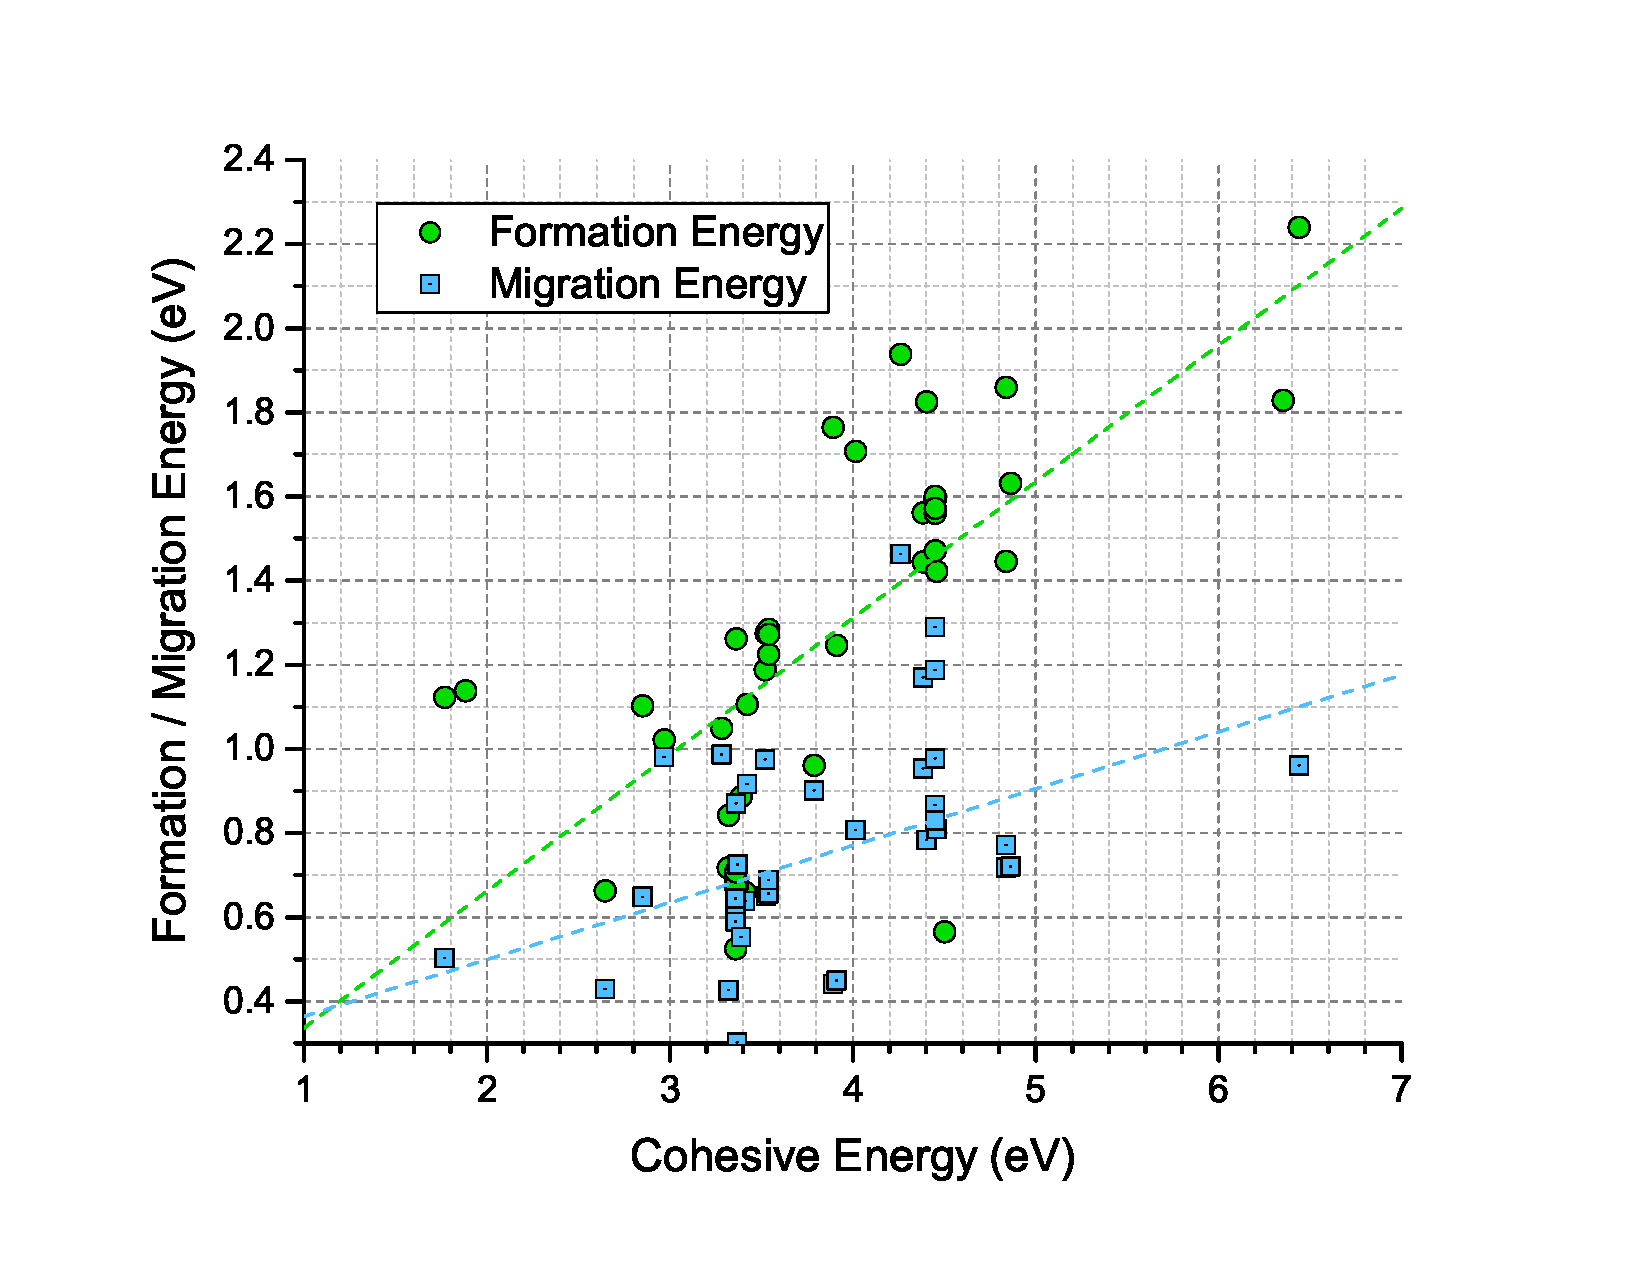
\includegraphics[width=0.5\textwidth, clip, trim = 10mm 10mm 10mm 10mm]{vfevme_vs_coh}% Here is how to import EPS art
\caption{\label{fig:vfevmevscoh}
Vacancy formation and migration energy versus cohesive energy.
These are calculated with EAM models for fcc structures.
As we can see, there is a linearly upward trend for both quantities.
The fitted slope for the formation energy and the migration energy are $0.32\pm0.04$ and $0.14\pm0.04$, respectively.
}
\end{figure}

Fig.~\ref{fig:vfevmevscoh} shows the relationship between the vacancy formation and migration energies and the cohesive energy.
We can see there is a linear increasing trend between the vacancy-related energies and the cohesive energy.
For the relationship between VFE and the cohesive energy, the slope is $0.32\pm0.04$, which agrees well with a previous DFT study, which gives a slope of $0.317$ \cite{angsten2014elemental}.
For the relationship between VME and the cohesive energy, the slope is $0.14\pm0.04$, which is also similar to the DFT result, $0.191$.

\begin{figure}
\centering
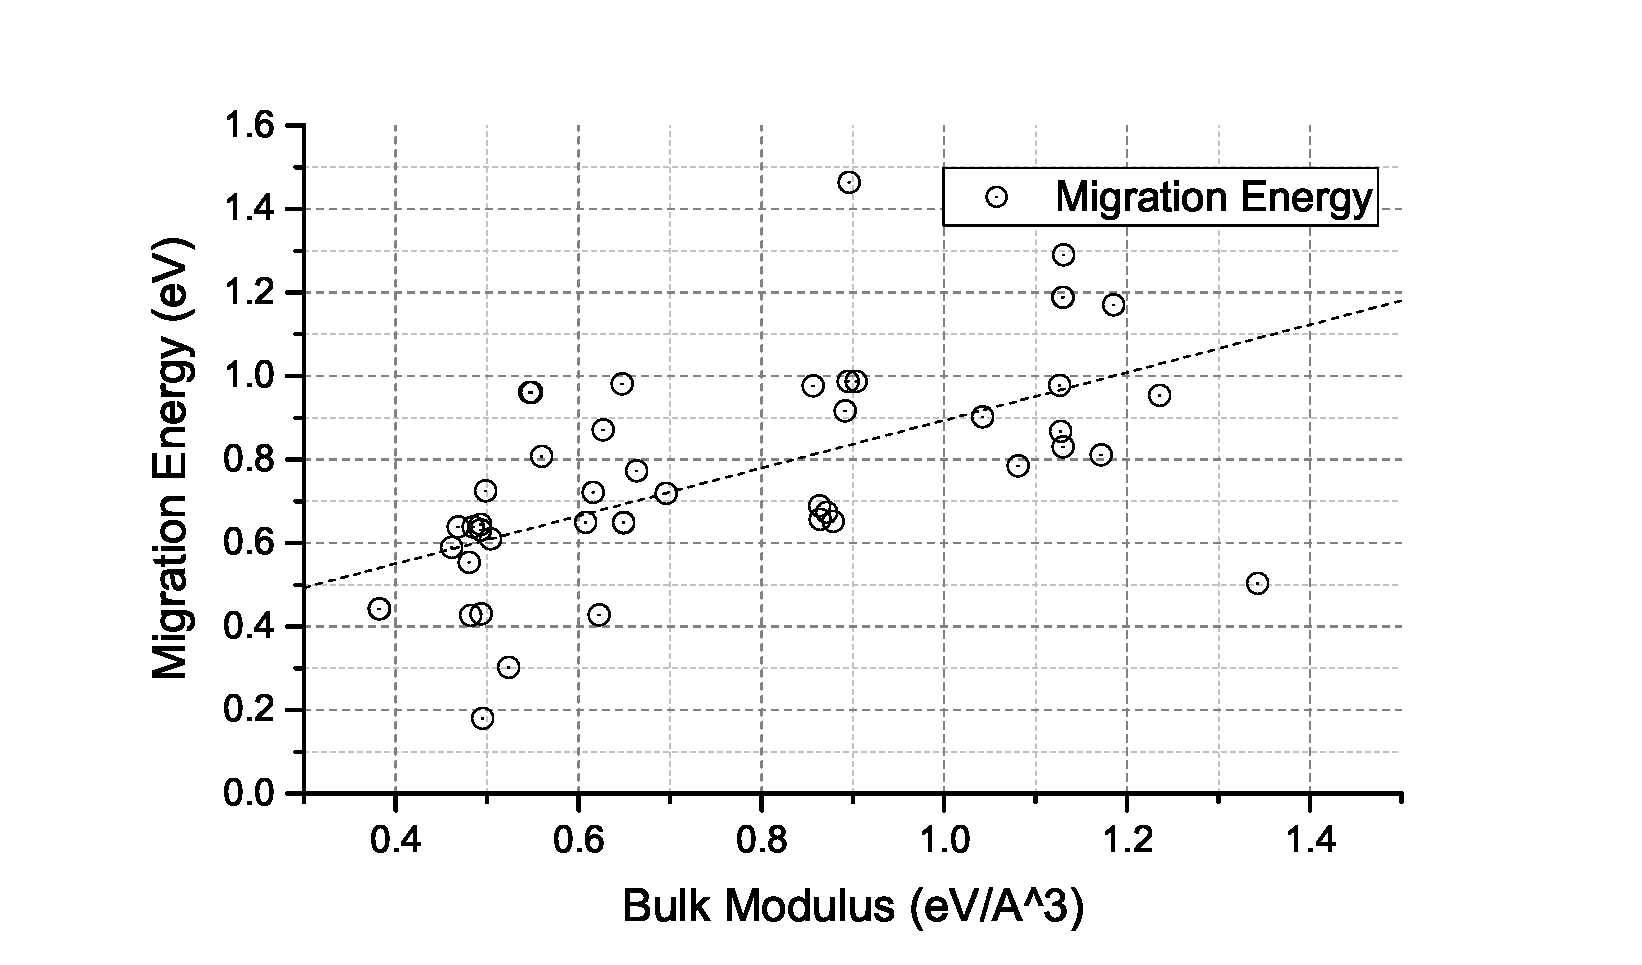
\includegraphics[width=0.5\textwidth, clip, trim = 10mm 3mm 10mm 10mm]{vme_vs_bulk}% Here is how to import EPS art
\caption{\label{fig:vmevsbulk}
Vacancy migration energy versus bulk modulus.
These are calculated with EAM models for fcc structures.
As we can see, there is a linearly upward trend.
The fitted slope and intercept are $(0.57\pm0.10)~\angstrom^3$ and $(0.32\pm0.08)~\electronvolt$, respectively.
}
\end{figure}

Fig.~\ref{fig:vmevsbulk} shows the relationship between the vacancy migration energy and the bulk modulus.
We can see there is also a linearly increasing trend.
The slope of the fitted line is $(0.57\pm0.10)~\angstrom^3 = (3.5\pm0.6)~\electronvolt\per\mathrm{GPa}$.
This result is quantitatively a little bit smaller than the DFT prediction, $5.5~\electronvolt\per\mathrm{GPa}$, but qualitatively still the same.

\begin{figure}
\centering
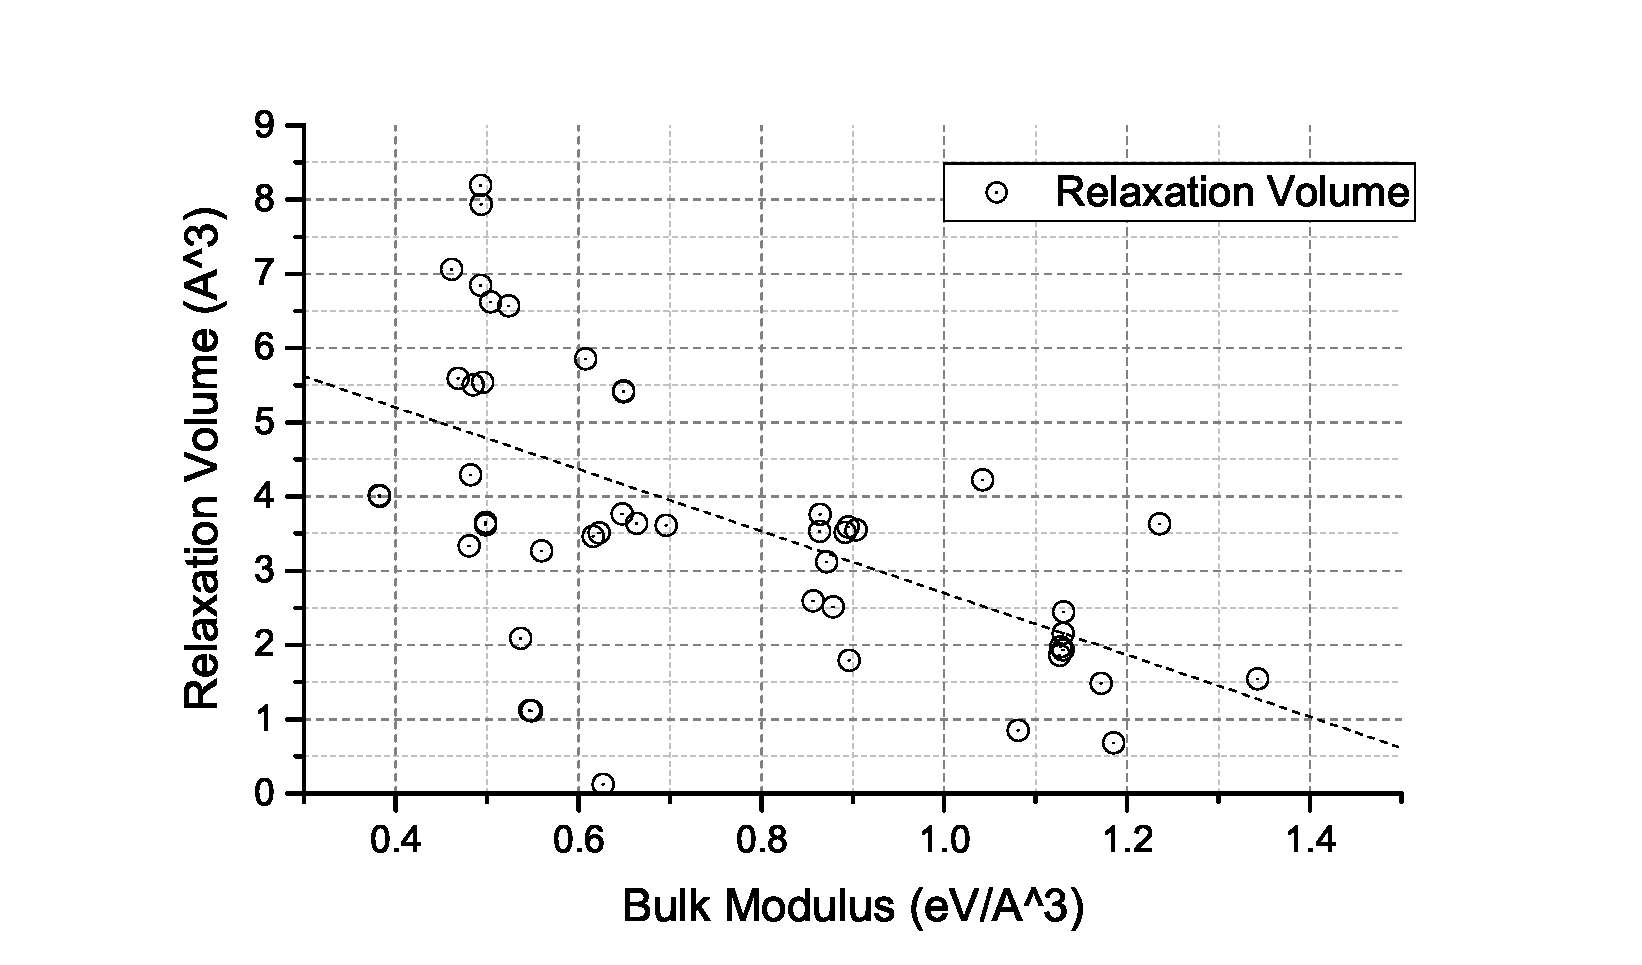
\includegraphics[width=0.5\textwidth, clip, trim = 10mm 3mm 10mm 10mm]{vrv_vs_bulk}% Here is how to import EPS art
\caption{\label{fig:vrvvsbulk}
Vacancy relaxation volume versus bulk modulus.
These are calculated with EAM models for fcc structures.
As we can see, there is a linearly downward trend.
The fitted slope and intercept are $(-4.2\pm0.7)~\angstrom^6\per\electronvolt$ and $(6.8\pm0.6)~\angstrom^3$, respectively.
}
\end{figure}

Fig.~\ref{fig:vrvvsbulk} shows the relationship between the vacancy relaxation volume and the bulk modulus.
% We expected that as the bulk modulus increases, the effect on the bulk strain due to the internal pressure created by the vacancy becomes smaller.
And we can see from the figure that there is a linear downward trend, which is consistent with the intuition that as the material becomes more stiff, the shrink due to the internal stress created by the vacancy decreases.
The slope of the fitted line is $(-4.2\pm0.7)~\angstrom^6\per\electronvolt$.

\begin{figure}
\centering
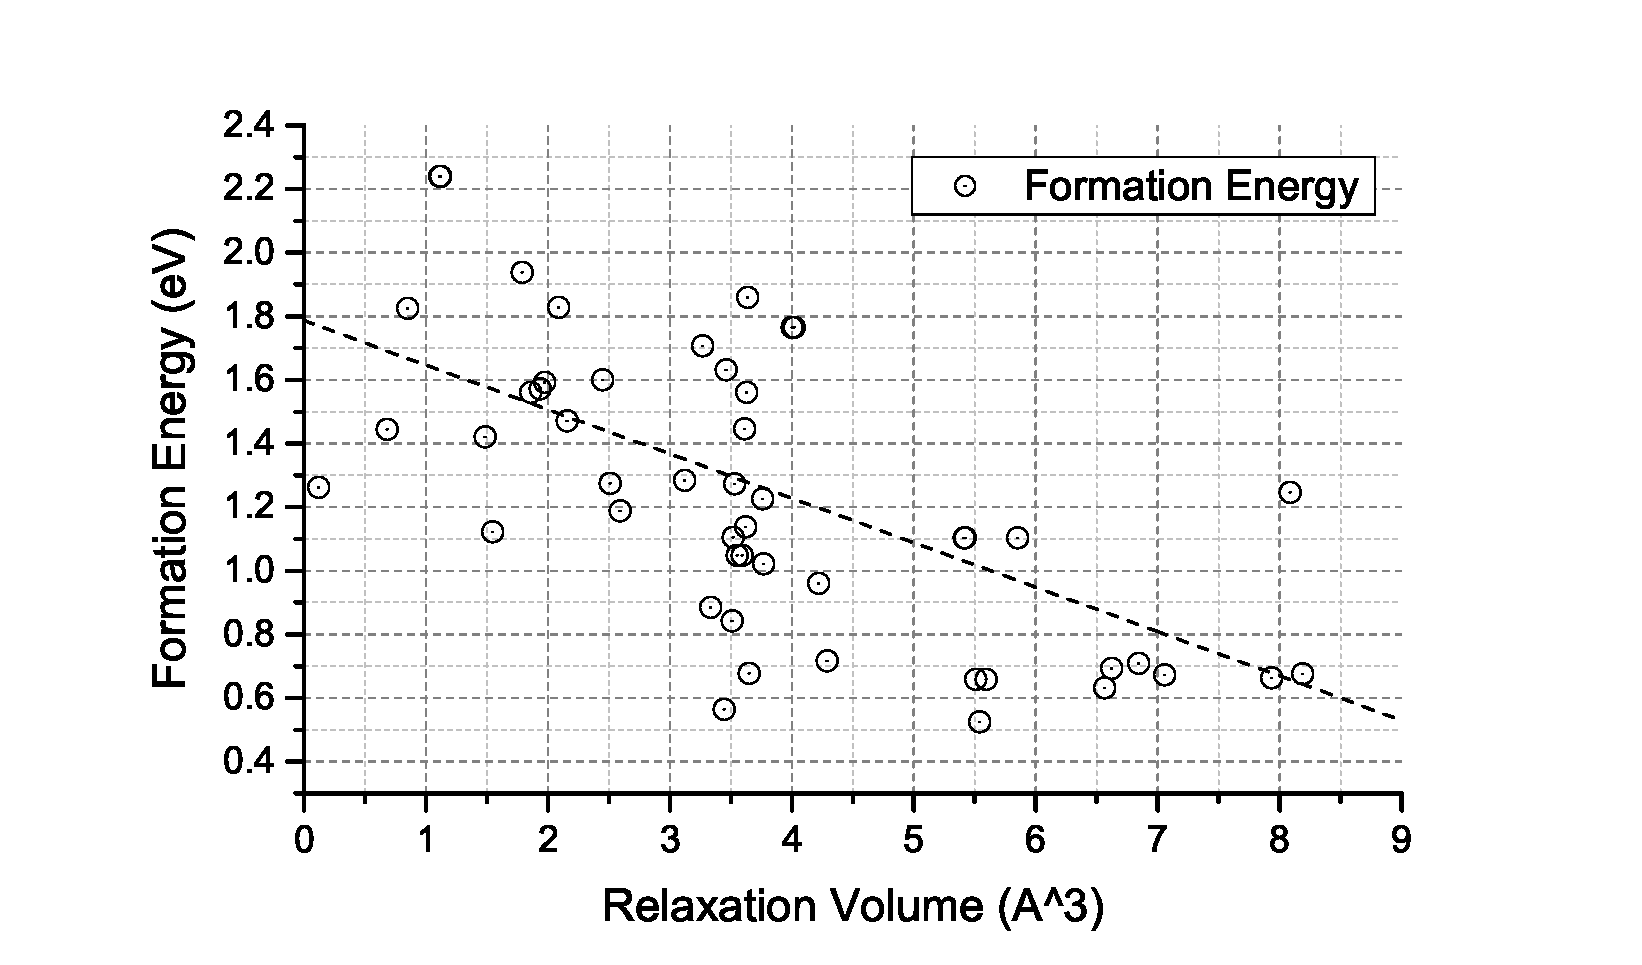
\includegraphics[width=0.5\textwidth, clip, trim = 10mm 3mm 10mm 10mm]{vfe_vs_vrv}% Here is how to import EPS art
\caption{\label{fig:vfevsvrv}
Vacancy formation energy versus relaxation volume.
These are calculated with EAM models for fcc structures.
As we can see, there is also a linearly downward trend.
The fitted slope and intercept are $(-0.14\pm0.02)~\electronvolt\per\angstrom^3$ and $(1.78\pm0.09)~\electronvolt$, respectively.
}
\end{figure}

We also found there is a strong correlation between the vacancy formation energy and the vacancy relaxation volume.
Fig.~\ref{fig:vfevsvrv} shows the relationship.
The slope of the fitted line is $(-0.14\pm0.02)~\electronvolt\per\angstrom^3$.
This downward trend is also consistent with the intuition that the energy needed for the vacancy to pull the neighboring atoms towards itself decreases with the help of additional bulk strain.

The results above are from fcc structures and the models available on OpenKIM at this time.
Appendix~\ref{app:data} provides Python scripts for retrieving the data from the OpenKIM repository, which can be used to obtain the relationships for all the structures with the latest data.

\section{\label{sec:conclusion}Conclusion}

In this study, we try to solve the problem of assessing the quality of interatomic models in terms of their ability to describe vacancy-related properties.

We developed tests using the OpenKIM API to perform atomistic calculations and obtain the most important monovacancy properties for all the simple structures and all the interatomic models in the OpenKIM repository at this time.

Then, we compare the calculated data with the reference data from DFT and experiments.
The results show that the EAM potentials, in general, agree with DFT calculations and experiments better than other kinds of potential models in the repository at this time.
The pairwise potentials tend to overestimate the vacancy formation energy for transition metals and post-transition metals.
One caveat to note is that neither the DFT results nor the experiments are assured to be accurate.
It is always beneficial to have more accurate and more comprehensive reference data from other sources with which to compare our results.

And finally, we looked into how these properties related to each other and to other elemental properties.
We got consistent results with physics intuition and previous studies, which further support the reliability of our results and these relationships.
These relationships can provide additional information for choosing models and screening structures.

%
% \begin{acknowledgments}
% We wish to acknowledge the support of the author community in using
% REV\TeX{}, offering suggestions and encouragement, testing new versions,
% \dots.
% \end{acknowledgments}

\appendix
\section{Point Defect Position Definition}
\label{app:position}
We model a point defect as a series forces exerted on neighboring atoms.
Let $\bm{F}^{v}$ be the body force exerted by the defect on atom $v$ situated at $\bm{l}^v$.
Then the displacement field can be written as
\begin{equation}
u_i(\bm{x}) = \sum_{v=1}^{N} g_{ij}(\bm{x}-\bm{l}^v) F_j^v
\end{equation}
$g_{ij}$ is the Green's function of a unit point force \cite{seifmultipolar,ting1997three}.

Expanding $u_i$ around an arbitrary point $\bm{x'}$, gives
\begin{multline}
u_i(\bm{x})
= g_{ij}(\bm{x}-\bm{x'}) P_j^{(0)}
 + \frac{\partial g_{ij}(\bm{x}-\bm{x'})}{\partial x_k'} P_{kj}^{(1)}\\
 + \frac{\partial^2 g_{ij}(\bm{x}-\bm{x'})}{\partial x_k' \partial x_l'} P_{klj}^{(2)}
 + \cdots
\end{multline}
Here $\bm{P}^{(k)}$ are the multipoles corresponds to $\bm{x'}$,
\begin{equation}
  P_j^{(0)} = \sum_{v=1}^N F_j^v = 0
\end{equation}
\begin{equation}
  P_{kj}^{(1)} = \sum_{v=1}^N (x'_k-l_k^v) F_j^v = \sum_{v=1}^N -l_k^v F_j^v
\end{equation}
\begin{align}
  P_{klj}^{(2)} & = \sum_{v=1}^N (x'_k-l_k^v) (x'_l-l_l^v) F_j^v \nonumber \\
  & = \sum_{v=1}^N l_k^vl_l^v F_j^v + x'_k P_{lj}^{(1)} + x'_l P_{kj}^{(1)}
\end{align}

$\bm{P}^{(1)}$ is the force dipole.
It is independent of the $\bm{x'}$ we choose.
Also, it is symmetric, because the torque on the system
\begin{equation}
  \tau_i = \sum_{v=1}^N l_j^v F_k^v - l_k^v F_j^v = -P_{jk}^{(1)} + P_{kj}^{(1)} = 0
\end{equation}
Therefore, $\bm{P}^{(1)}$ is diagonalizable.

$\bm{P}^{(2)}$ depends on the choice of $\bm{x'}$.
Although we can perform multipole expansion with respect to any $\bm{x'}$, we hope our choice of $\bm{x'}$ can give a direct impression of where the defect is situated.
Therefore, we propose using the following criteria:
choose $\bm{x'}$ such that, in the basis where $\bm{P}^{(1)}$ is a diagonal matrix,
\begin{equation}
  P_{iii}^{(2)} = \sum_{v=1}^N (x'_i-l_i^v)^2 F_i^v = 0
\end{equation}
This gives an unambiguous definition for $\bm{x'}$ and also makes $\bm{x'}$ the center of the forces.
And it is consistent with the case where the symmetry is preserved.

\section{Obtaining Results From OpenKIM}
\label{app:data}
The results can be obtained either via the web interface directly \url{https://openkim.org/intro-tests/} or through OpenKIM Query \url{query.openkim.org}.
We describe the later one in this section.

OpenKIM Query works for any programming languages as long as they support HTTP requests.
We use Python here as an example.
The backend of this query API is a MongoDB database, and in order to obtain the results we want, we need to construct our query with the correct MongoDB syntax.
The website of MongoDB, \url{mongodb.org}, provides a detailed documentation of this.

Here is an example of using Python to obtain all the fcc aluminum lattice constants (TODO: replace by vacancy formation energy) calculated with various interatomic potentials:
\begin{lstlisting}
import requests
res = requests.get('https://query.openkim.org/api?flat=on&query={"meta.type":"tr","property-id":"tag:staff@noreply.openkim.org,2014-04-15:property/structure-cubic-crystal-npt","meta.runner.kimcode":{"$regex":"^LatticeConstantCubicEnergy_fcc"},"species.source-value":"Al"}&limit=0&fields={"a.source-value":1,"meta.subject.kimcode":1}&database=data').json()
\end{lstlisting}

To obtain a plot of lattice constant versus bulk modulus for all the models and all the elements, we can do
\begin{lstlisting}
import requests
import pandas as pd
import matplotlib.pyplot as plt

# Obtain data
res_lat = pd.read_json('https://query.openkim.org/api?flat=on&query={"meta.type":"tr","property-id":"tag:staff@noreply.openkim.org,2014-04-15:property/structure-cubic-crystal-npt","meta.runner.kimcode":{"$regex":"^LatticeConstantCubicEnergy_fcc"}}&limit=0&fields={"a.source-value":1,"species.source-value":1,"meta.subject.kimcode":1}&database=data')
res_bulk = pd.read_json('https://query.openkim.org/api?flat=on&query={"meta.type":"tr","property-id":"tag:staff@noreply.openkim.org,2014-04-15:property/bulk-modulus-isothermal-cubic-crystal-npt","meta.runner.kimcode":{"$regex":"^ElasticConstantsCubic_fcc"}}&limit=0&fields={"isothermal-bulk-modulus.source-value":1,"meta.subject.kimcode":1,"species.source-value":1}&database=data')

# Merge on species and model name
res_lat['species'] = res_lat['species.source-value'].apply(lambda x: x[0])
res_bulk['species'] = res_bulk['species.source-value'].apply(lambda x: x[0])
res = pd.merge(res_lat, res_bulk, how = 'inner', on = ['meta.subject.kimcode', 'species'])

# Remove outliers
bulk = res['isothermal-bulk-modulus.source-value']
res_cleaned = res[(bulk > 0) & (bulk < 1000)]

# Plot
res_cleaned.plot(x = 'a.source-value', y = 'isothermal-bulk-modulus.source-value', style = 'o')
plt.show()
\end{lstlisting}

We can also perform a linear regression with the data obtained above
\begin{lstlisting}
from pandas.stats.api import ols
ols(y = res_cleaned['isothermal-bulk-modulus.source-value'], x = res_cleaned['a.source-value'])
\end{lstlisting}
The code above has been tested in the Python 2.7 version of Anaconda 4.0.0.





%Note the equation numbers in this appendix, produced with the
%subequations environment:
%\begin{subequations}
%\begin{eqnarray}
%E&=&mc, \label{appa}
%\\
%E&=&mc^2, \label{appb}
%\\
%E&\agt& mc^3. \label{appc}
%\end{eqnarray}
%\end{subequations}
%They turn out to be Eqs.~(\ref{appa}), (\ref{appb}), and (\ref{appc}).

% The \nocite command causes all entries in a bibliography to be printed out
% whether or not they are actually referenced in the text. This is appropriate
% for the sample file to show the different styles of references, but authors
% most likely will not want to use it.
\nocite{*}

\bibliography{vacancy}% Produces the bibliography via BibTeX.

\end{document}
%
% ****** End of file apssamp.tex ******
